\section{Theory}
\label{sec:theory}
The theory is splitted into X sections the LHCb in general in \autoref{sec:LHCb}.
\subsection{Large Hadron Collider beauty}
\label{sec:LHCb}

\begin{figure}[h]
    \centering
    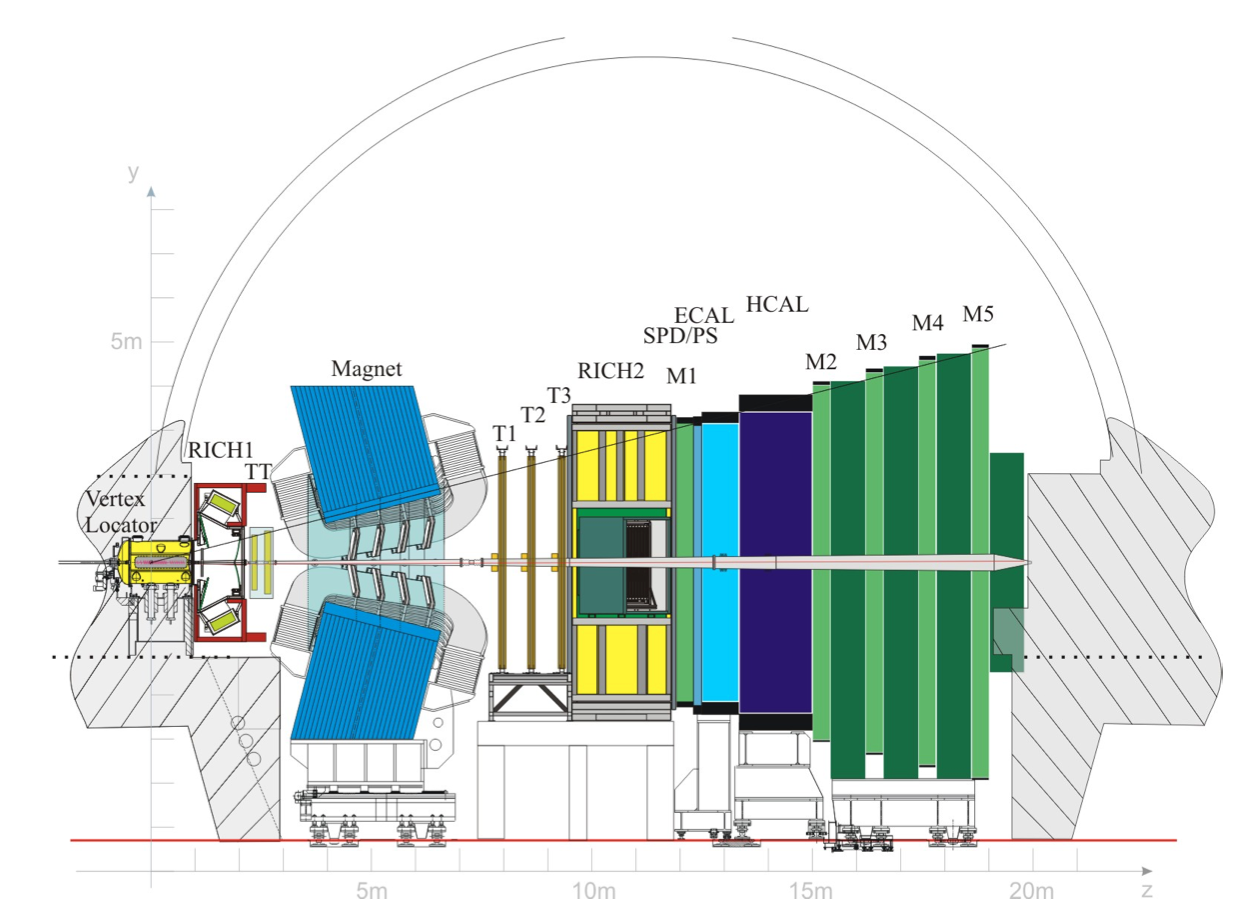
\includegraphics[width=\textwidth]{content/Figures/LHCb.png}
    \caption[Schematic view of the LHCb detector in Run 1.]
    {Schematic side view of the LHCb detector and its main subdetectors
    during Run 1 \cite{CPVVorlage}.}
    \label{fig:LHCb}
\end{figure}

The LHCb detector is constructed as a single-arm forward spectrometer,
because the production of $b$-$\bar{b}$ pairs in $pp$ collisions is strongly
peaked at small angles relative to the beam axis.
Therefore, many of the resulting $b$ hadrons enter the forward acceptance
of the LHCb detector \cite{TDR}.

In Figure \ref{fig:LHCb}, the LHCb detector configuration used during Run 1
is shown.
The \textit{Vertex Locator} (VELO) is used to identify and distinguish the
primary and secondary vertices of the particles.
Since these are only a few millimetres apart,
the VELO is located directly around the interaction point.
Together with the \textit{Trigger Tracker} (TT),
the \textit{dipole magnet} and the tracking stations T1, T2 and T3,
the VELO forms the tracking system of LHCb.
The tracking stations consist of the \textit{Inner Tracker} (IT)
and the \textit{Outer Tracker} (OT).
This system is used to reconstruct particle tracks and to determine the
momentum, which can be obtained from the deflection of charged particles
in a magnetic field.

The detectors \textit{RICH1}, \textit{RICH2}, the calorimeter system and the
muon stations \textit{M1} to \textit{M5} are used for particle identification.
The focus here is on distinguishing pions, kaons and protons,
as well as electrons, photons and muons,
because they are common decay products of $b$ hadrons \cite{TDR}.
The RICH detectors are used to distinguish charged hadrons,
especially pions, kaons and protons.
They measure the Cherenkov light emitted by charged particles and combine
this information with the measured momentum of the track.
This allows LHCb to assign a particle hypothesis to each reconstructed track.

This is essential for $B$-decay analyses,
because the final-state particles must be identified correctly.
In the decay $\text{B}^+ \to K^+K^-K^+$, for example,
all three charged tracks have to be identified as kaons.
A pion that is misidentified as a kaon is an important source of background.
Since the assumed particle mass is used to calculate the particle energy,
a wrong particle identification changes the reconstructed invariant mass
of the $B^+$ candidate.
Such misidentified events can therefore contribute to the background of the
selected signal.

The calorimeter system consists of the \textit{Scintillating Pad Detector}
(SPD), the \textit{Preshower Detector} (PS),
the \textit{Electromagnetic Calorimeter} (ECAL) and the
\textit{Hadronic Calorimeter} (HCAL).
The calorimeters identify photons, electrons and hadrons,
while the muon stations identify muons.
Together with the tracking system, these detectors allow the full
reconstruction and classification of the decay products of $b$ hadrons.